\chapter[Quantum Chromodynamics (QCD): A Picture Book]{Quantum Chromodynamics:\\A Picture Book}
\markboth{\small \textsc{Chapter \thechapter}: \bf QCD: A Picture Book}{}

\label{chap:picturebook}

\epigraph{Never trust an atom: they make up everything.}{An atom}

\epigraph{There are more things in Heaven and Earth, Horatio, than are dreamt of in your philosophy.}{Shakespeare, \underline{Hamlet}}


70 years ago, humanity discovered new particles that nobody expected.
%
Dozens of them.
%
After the conceptualization of molecules in the 19\th{} century, atoms in the 20\th{} century, and the even smaller protons, neutrons, electrons, muons, and neutrinos, you may have thought we had seen the building blocks of everything under the sun.
%
But we hadn't.

The discovery of the zoo of new particles -- what we called the \(\Delta\), the \(K^*\), the \(\rho\), and scores of others -- showed us that everything we knew was not enough.
%
The next 20 years saw a bedlam of earnest confusion, controversy, and adventure in the field of particle physics, as humanity desperately strove to understand the moves of over one hundred new chess pieces.
%
The all-encompassing framework of \gls{qft}, the great unifying language of modern physics, faltered.
%
By the 1960s, it teetered on the edge of irrelevance -- mocked, dismissed, almost forgotten.
%
Nearly consigned to oblivion, \gls{qft} seemed to raggedly breathe its last.

\textit{Then, it came roaring out of its deathbed in triumph.}

Hidden in the chaos of hundreds of numbers -- masses, charges, decay rates -- lay a deep order glimpsed by Gell-mann \cite{Gell-Mann:1964ewy} and Zweig \cite{Zweig:1964ruk,Zweig:1964jf} in their quark model, and in the geometric theory of Yang and Mills \cite{Yang:1954ek}, which forged together into the theory of \gls{qcd}.
%
In radical defiance of the theorists of the previous generation, Politzer \cite{Politzer:1973fx} and Gross and Wilczek \cite{Gross:1973ju} discovered that QCD was one of the only quantum field theories invulnerable to the disparagements of their predecessors.
%
We had obtained a theory of the strong force;
%
a theory that overcame decades of confusion, and explained our unexpected observation of dozens of new particles.

\textit{The mystery of the particle zoo was the manifestation of the symmetries of QCD.}


\vspace{1.5cm}
\hrule
\begingroup

\setlength \epigraphwidth {\textwidth}
\setlength \epigraphrule {0pt}
\renewcommand {\epigraphflush} {center}
\renewcommand {\sourceflush} {center}

\epigraph{
        When you ask what are electrons and protons I ought to answer that this question is not a profitable one to ask and does not really have a meaning.
    %
    The important thing about electrons and protons is not what they are but how they behave, how they move.
    %
    I can describe the situation by comparing it to the game of chess.
    %
    In chess, we have various chessmen [sic], kings, knights, pawns and so on.
    %
    If you ask what a chessman is, the answer would be that it is a piece of wood, or a piece of ivory, or perhaps just a sign written on paper, or anything whatever.
    %
    It does not matter.
    %
    Each chessman has a characteristic way of moving and this is all that matters about it.
    %
    The whole game of chess follows from this way of moving the various chessmen.
}{---Paul Adrien Maurice Dirac}

\endgroup

\vspace{0.2cm}
\hrule
\vspace{1.5cm}


As we explored our universe, it slowly became clear that QCD described the inner lives of many of the particles we saw.
%
Just as Rutherford beheld the astounding result that atoms had an inner structure formed by protons and neutrons in the early 20\th{} century, the experiments of the late 20\th{} century showed that protons and neutrons were themselves made of more fundamental pieces.

Feynman named the new chess pieces partons, Gell-mann named them quarks and gluons, and we began to understand that they composed protons, neutrons, and the dozens of new particles of the particle zoo.
%
But we saw something even more curious.
%
When we tried to produce quarks in particle collisions, evidence began to suggest that \textit{they themselves were composed of quarks}.
%
The experimental data matched the prediction that a single energetic quark or gluon produced in a particle collision underwent a dramatic fragmentation into many more partons.
%
In fact, the theory of QCD seemed to suggest that a single quark or gluon contained an \textit{infinite number of partons within}.

Luckily, Sterman and Weinberg discovered a way around the divergences of QCD \cite{Sterman:1977wj};
%
they predicted that the chess pieces of QCD at high energies, not unlike the water droplets spraying from a high pressure hose, should shower into \vocab{jets} each potentially containing dozens of particles or more.
%
The jets they predicted as proxies for the high energy quarks and gluons produced by colliding particles were soon measured \cite{Hanson:1975fe,Wiik:1979cq,Barber:1979yr,TASSO:1979zyf,PLUTO:1979dxn,JADE:1979rke,Ali:1979em,Hanson:1981em,Ali:2010tw}, and the explosion of experimental, phenomenological, and theoretical study of jets that followed solidified \gls{qcd} as our fundamental theory of the strong nuclear force.
%
It is not an exaggeration to say that the discovery of jets has been one of the most important developments in the history of our study of the natural world.

By studying the correlations of hadronic radiation within jets, we may probe their internal structure and gain even more information about the \gls{sm}, \gls{qcd}, and beyond.
%
However, the substructure of jets is difficult to predict, especially through the obfuscating haze of additional particles that accompany jets in the messy environment of particle collisions.
%
We must design jet substructure observables which are both experimentally meaningful and experimentally calculable, and are robust to the effects of the addition pollution produced by particle collisions.

\textit{To understand the most fundamental known building blocks of our universe, we must study the substructure of jets.}
%
\textbf{\textit{Designing robust probes to expose the fractal-like, inner life of jets through a haze of contaminating radiation is the subject of this thesis.}}



\begin{figure}[]
    {
        \hspace{-1.7cm}
        \begin{tikzpicture}[very thick]
    % Define coordinate transformation function
    \pgfmathsetmacro{\compressfactor}{1}
    \pgfmathsetmacro{\earlytransition}{1947}
    \pgfmathsetmacro{\moderntransition}{1973}

    \tikzset{
        my coords/.style={
            x={0.25cm},
            y={1cm},
        }
    }

    \begin{scope}[my coords]
        % Colors
        \definecolor{particleera}{RGB}{255,240,230}
        \definecolor{modernera}{RGB}{230,255,230}
        \definecolor{particledot}{RGB}{255,200,180}
        \definecolor{moderndot}{RGB}{180,255,180}
        \definecolor{particleoutline}{RGB}{255,140,100}
        \definecolor{modernoutline}{RGB}{50,180,50}

        % New colors for event types
        \definecolor{theorycol}{RGB}{100,140,255}
        \definecolor{experimentcol}{RGB}{255,100,100}
        \definecolor{particlecol}{RGB}{180,100,255}
        \definecolor{milestonecolor}{RGB}{100,40,120}

        % Styles
        \tikzset{
            experiment/.style={diamond, fill=experimentcol!80, draw=experimentcol!70!black, line width=0.8pt, inner sep=1.5pt},
            theory/.style={rectangle, fill=theorycol!80, draw=theorycol!70!black, line width=0.8pt, inner sep=2pt},
            particle/.style={circle, fill=particlecol!80, draw=particlecol!70!black, line width=0.8pt, inner sep=2pt},
            milestone/.style={particle}, % Now just using particle style for milestones
            exp label/.style={text width=2.8cm, align=center, font=\scriptsize},
            theory label/.style={text width=2.8cm, align=center, font=\scriptsize, rotate=-40},
            particle label/.style={text width=2.8cm, align=center, font=\scriptsize}
        }

        % Era backgrounds
        \fill[draw=white, left color=particleera!15, middle color=particleera, right color=particleera!90!modernera] (\earlytransition,2.4) rectangle (\moderntransition,-2.6);
        \fill[draw=white, left color=modernera!90!particleera, middle color=modernera, right color=modernera!15] (\moderntransition,2.4) rectangle (2012,-2.6);

        % Main timeline
        \draw[line width=1.2pt] (1947,0) -- (2012,0);

        % Era labels
        \node[font=\small\itshape] at (1960,2.8) {Pre-QCD Era};
        \node[font=\small\itshape] at (1996.5,2.8) {Era of QCD and the Standard Model};

        % Tick marks
        \foreach \year in {1950,1960,1970,1980,1990,2000,2010} {
            \draw (\year,-0.2) -- (\year,0.2);
            \node[below=0.05cm, font=\tiny] at (\year,-0.2) {\year};
        }

        % PARTICLE DISCOVERIES (placed at y=0 with vertical offsets and horizontal labels)

        % Pion (now a regular particle)
        \node[particle] (pion) at (1947,0) {};
        \node[particle label] at (1947,0.6) {\textbf{1947}\\$\pi$ (Pion)};

        % Strange particles
        \node[particle] (strange) at (1953,0) {};
        \node[particle label] at (1953,0.8) {\textbf{1953}\\Strange\\particles};

        % Omega-minus
        \node[particle] (omega) at (1964,0) {};
        \node[particle label] at (1964,0.6) {\textbf{1964}\\$\Omega^-$};

        % J/psi
        \node[particle] (jpsi) at (1974,0) {};
        \node[particle label] at (1974,0.6) {\textbf{1974}\\J/$\psi$};

        % Upsilon (added)
        \node[particle] (upsilon) at (1977.5,0) {};
        \node[particle label] at (1977.5,0.6) {\textbf{1977}\\$\Upsilon$};

        % W and Z bosons (added)
        \node[particle] (wz) at (1983.5,0) {};
        \node[particle label] at (1983.5,0.6) {\textbf{1983}\\$W$ and $Z$};

        % Top quark (added)
        \node[particle] (top) at (1995.5,0) {};
        \node[particle label] at (1995.5,0.6) {\textbf{1995}\\Top quark};

        % Higgs boson (now a regular particle)
        \node[particle] (higgs) at (2012,0) {};
        \node[particle label] at (2012,0.6) {\textbf{2012}\\Higgs boson};

        % EXPERIMENTAL EVENTS

        % DIS at SLAC (stays above)
        \node[experiment] (dis) at (1969,0) {};
        \draw[-, dashed] (dis) -- (1969,1.0);
        \node[exp label] at (1969,1.5) {\textbf{1969}\\Deep Inelastic\\Scattering (SLAC)};

        % Jets at UA1/UA2 (stays above)
        \node[experiment] (jets-exp) at (1983,0) {};
        \node[exp label] at (1983,1.6) {\textbf{1983}\\Jets observed\\at UA1/UA2};

        % Moved to bottom row
        % Gluon jets (MOVED to bottom)
        \node[experiment] (gluon) at (1979,0) {};
        \draw[-, dashed] (gluon) -- (1979,-1.3);
        \node[theory label] at (1979,-1.85) {\textbf{1979}\\Gluon jets\\(PETRA)};

        % LEP precision (MOVED to bottom)
        \node[experiment] (lep) at (1989,0) {};
        \draw[-, dashed] (lep) -- (1989,-1.0);
        \node[theory label] at (1989,-1.6) {\textbf{1989}\\QCD precision\\tests (LEP)};

        % Quark-gluon plasma (MOVED to bottom)
        \node[experiment] (qgp) at (2000,0) {};
        \draw[-, dashed] (qgp) -- (2000,1.0);
        \node[exp label] at (2000,1.5) {\textbf{2000}\\Quark-gluon\\plasma (RHIC)};

        % THEORETICAL EVENTS (below the line)

        % Eightfold Way
        \node[theory] (eightfold) at (1961,0) {};
        \draw[-, dashed] (eightfold) -- (1961,-0.8);
        \node[theory label] at (1961,-1.3) {\textbf{1961}\\Eightfold Way};

        % Parton model
        \node[theory] (parton) at (1967,0) {};
        \draw[-, dashed] (parton) -- (1967,-0.8);
        \node[theory label] at (1967,-1.3) {\textbf{1967}\\Parton model};

        % Asymptotic freedom
        \node[theory] (qcd) at (1973,0) {};
        \draw[-, dashed] (qcd) -- (1973,-1.0);
        \node[theory label] at (1973,-1.5) {\textbf{1973}\\Asymptotic freedom};

        % Jets defined
        \node[theory] (jets-theory) at (1976.7,0) {};
        \draw[-, dashed] (jets-theory) -- (1976.7,-0.2);
        \node[theory label] at (1976.3,-0.7) {\textbf{1977}\\Jets defined};

        % Jet substructure
        \node[theory] (substructure) at (2005,0) {};
        \draw[-, dashed] (substructure) -- (2005,-1.0);
        \node[theory label] at (2005,-1.6) {\textbf{2005}\\Jet substructure\\revolution};


        % Simplified Legend
        \begin{scope}[shift={(2017,0.0)}]
            \node[particle, anchor=west] at (0,1.0) {};
            \node[anchor=west, align=center, font=\scriptsize] at (2.0,1.0) {Particle\\Discovery};

            \node[experiment, anchor=west] at (0,0.0) {};
            \node[anchor=west, align=center, font=\scriptsize] at (1,0.0) {Experimental\\Result};

            \node[theory, anchor=west] at (0,-1.0) {};
            \node[anchor=west, align=center, font=\scriptsize] at (1,-1.0) {Theoretical\\Development};
        \end{scope}
    \end{scope}
\end{tikzpicture}

    }
    \caption[A rough timeline of the history of \gls{qcd}. \sam{incomplete}]
    {
        A rough timeline of the history of \gls{qcd}.
        %
        \sam{Not complete! Many particles, as well as QGP, missing! May want to change notation, e.g. for particle discoveries}
        %
        \sam{Noah recommends lines connecting things to dates...}
    }
    \label{fig:qcd-timeline}
\end{figure}


\vspace{1.0cm}
\hrule
\vspace{1.0cm}


Why should we care about the particle zoo?
%
Why should we care about the overwhelming experimental verification of a theory which describes the most fundamental known building blocks of our universe?
%
Why should we deeply explore and understand the predictions of this theory?
%
I can think of at least three answers:

\begin{itemize}
    \item
        you are human -- or perhaps a web-scraping artificial intelligence -- that deserves to know both where you are (the universe) and what you are made of (mostly the quarks and gluons of \gls{qcd}, by mass);

    \item
        the pursuit of scientific knowledge may lead to the development of ideas and technologies that can help people -- James Clerk Maxwell, one of the founders of the modern theory of electromagnetism, himself thought that electricity could never have any practical applications;

    \item
        gosh darn it, learning this stuff is really freaking fun.
\end{itemize}

Regarding the second point, I wish you luck with all my heart.
%
Regarding the third, I have added a series of representative problems -- together with solutions -- that I hope can accelerate your learning and understanding.

The first point speaks to me most deeply.


% -----------------------------------
% Particles Section:
% -----------------------------------
\begin{sourcefigure}[t!]
    % Figure graphics
    \centering
    \includegraphics[width=\textwidth]{example-image-a}

    % Caption
    \caption[A cartoon of the ideas of renormaliztion, in the context of zooming in from the largest to the smallest scales of the universe.]{
        A cartoon depicting zooming in on the universe, beginning at the largest known scales and ending at some of the smallest -- the scales of \gls{qcd}.
        %
        The top row, from right to left, depicts galactic filaments, galaxies, and the solar system.
        %
        The middle row depicts terrestrial scales (right to left):
        %
        the earth, a hunk of iron, the magnetic domains within iron, and a single iron atom.
        %
        The bottom row depicts the scales of \gls{qcd} (right to left):
        %
        a proton, a jet, a partonic splitting, and a single quark.
    }
    % Figure Label
    \label{fig:picturebook_universe}
\end{sourcefigure}



% -----------------------------------
% Particles Section:
% -----------------------------------
\begin{sourcefigure}[t!]
    % Figure graphics
    \centering
    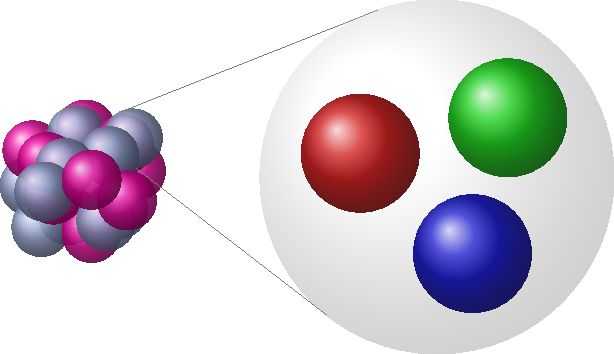
\includegraphics[width=0.65\textwidth]{figures/picturebook/particles}
    % Caption
    \caption[A visualization of quarks as fundamental particles within the proton.]{
        Quarks, visualized as red, blue, and green spheres, are fundamental particles contained within the proton.
        %
        This is only a visualization -- quarks are pointlike, as far as we know, and among the smallest known pieces of our universe.
    }
    % Figure Label
    \label{fig:picturebook_particles}
\end{sourcefigure}


% -----------------------------------
% Jets Section:
% -----------------------------------
\begin{sourcefigure}[t!]
    % Figure graphics
    \centering
    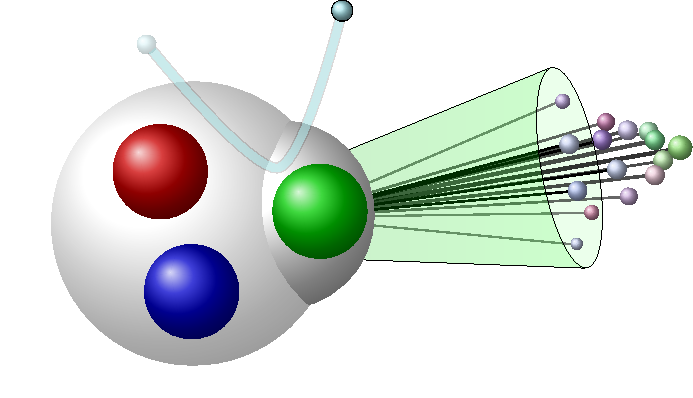
\includegraphics[width=0.6\textwidth]{figures/picturebook/dis-1}
    \hfill
    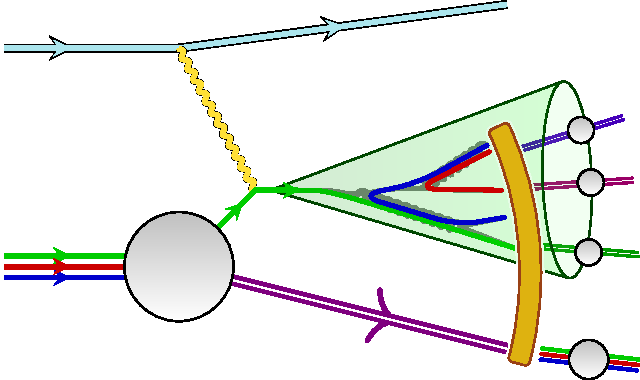
\includegraphics[width=0.6\textwidth]{figures/picturebook/dis-2}

    % Caption
    \caption[A visualization of jets formed by ejecting a quark from a nucleon during high energy scattering.]{
        Jets, collimated sprays of hadronic particles visualized as green cones, are formed when quarks (or gluons) are pushed out of their confines during a high-energy particle collision and undergo a cascading series of ``decays'' called the partonic cascade.
        % https://indico.cern.ch/event/492098/contributions/1169736/attachments/1356309/2050123/QCD2.pdf#page=21
    }

    % Figure Label
    \label{fig:picturebook_jets}
\end{sourcefigure}


% -----------------------------------
% Substructure Section:
% -----------------------------------
\begin{sourcefigure}[t!]
    % Figure graphics
    \centering
    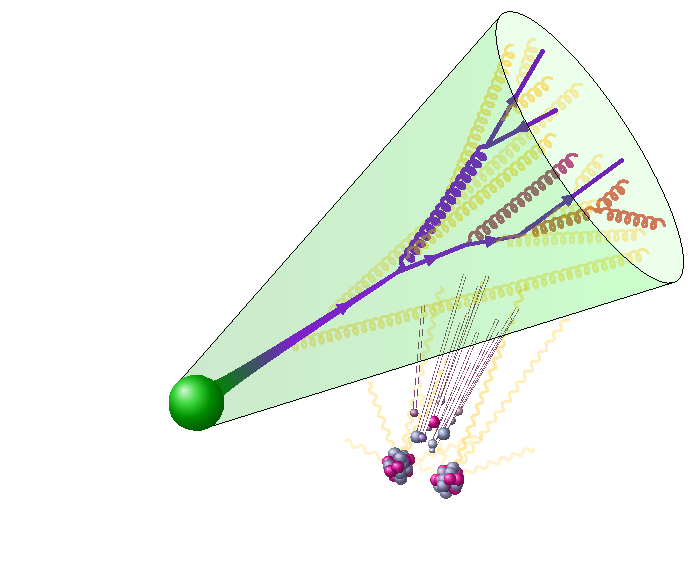
\includegraphics[width=0.8\textwidth]{figures/picturebook/jet-contamination}

    % Caption
    \caption[A visualization of the low-energy contamination within jets, whose removal is the goal of jet grooming.]{
        The goal of \emph{jet grooming} is to recover the information of high-energy jet substructure representing the physics of high energy quarks and gluons (visualized as dark, opaque lines, with darker colors/more opacity indicating higher energy) despite obfuscation from soft distortions (hadronization, detector effects) and additive contamination (pileup, underlying event).
    }

    % Figure Label
    \label{fig:picturebook_substructure}
\end{sourcefigure}


% -----------------------------------
% Event Shapes Section:
% -----------------------------------
\begin{sourcefigure}[t!]
    % Figure graphics
    \centering
    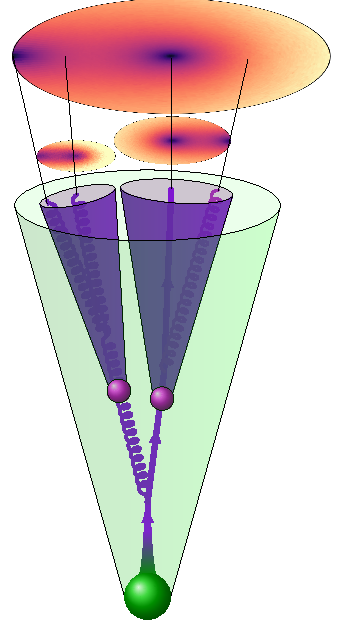
\includegraphics[width=0.38\textwidth, angle=-50]{figures/picturebook/fractal-substructure}

    % Caption
    \caption[A visualization of energy-weighted correlations capturing correlations between different high-energy structures within jets at different scales. \sam{incomplete, want bunch crossings rather than nuclei}]{
        Energy-weighted correlators capture correlations between high-energy structures within jets, such as particles (purple/black lines) or subjets (purple cones).
        %
        The explicit example of the resolved 3-point energy correlators of \Chap{ewocs}, compute using real collider data, are shown as colored disks above the jet to visualize energy-weighted correlations at different angular scales.
        %
        The higher energy regions of the cartoon jet depicted here are represented by higher values of the associated resolved energy correlator, and darker colors in the associated colored disks.
        %
        \sam{incomplete, want bunch crossings rather than nuclei}
    }
    % Figure Label
    \label{fig:picturebook_eventshapes}
\end{sourcefigure}




The story of \gls{qcd} is tightly intertwined with the story of \textit{renormalization} -- the way physical phenomena change as a function of scale.
%
It gives us a powerful framework for understanding how large structures emerge from smaller pieces, and we will barely scratch its incredibly vast implications in this thesis -- not for lack of trying!

Let's get our bearings.
%
As in \Fig{picturebook_universe}, we will zoom in on the universe from the largest scales to the smallest.
%
The largest, super-galactic structures we know of in the universe -- galactic filaments larger than 1 billion light years in length, \(10^{25}\) times larger than the \(\mathcal{O}(1 \text{ meter})\) macroscopic objects of our daily lives -- are composed of smaller pieces:
%
superclusters, then clusters, then groups of galaxies.
%
The ``small'' galaxies themselves tend to have a size of ``only'' \(10^{20}\) meters.
%
Our solar system is around \(10^{12}\) meters in size and our gorgeous planet earth only around \(10^7\) meters.
%
The vast separation of these scales -- the super-galactic, the galatic, the terrestrial -- is an amazing and curious feature:
%
the piecing together of small structures occurs at distances far larger than any individual piece could hope to traverse or understand.



The small structures themselves, however, are also immensely complicated.
%
The surface of the earth alone is home to an unimaginable number of ecological systems.
%
Each human home has an intricate and beautiful story.

And we ourselves are not the end.
%
Cells (for humans, \(10^{-4}\)-\(10^{-5}\) m), within them atoms (for hydrogen, around \(10^{-10}\) m) -- and protons, neutrons (\(10^{-18}\) m), electrons (pointlike, as far as we know) -- are the building blocks of our experience.

This thesis is a (\textit{very}) short sentence in the grand tale of the smallest scales we have been able to study with the scientific method%
\footnote{
    Don't tell the string theorists and quantum gravitists -- they have been able to probe even deeper with the power of pure thought!
}.
%
Like the largest scales of the known universe, the quarks and gluons within protons and neutrons, described by \gls{qcd}, are the smallest pieces we can experimentally probe.
%
They are the limits to our fundamental understanding of the universe.

The theory of \gls{qcd} describes over \(99.9\%\) of the visible mass of the universe, and therefore the majority of what we might see if we were able to zoom deeply into the structures of the macroscopic objects of our daily experience.%
\footnote{
    The mass of the hydrogen atom, for example, is more than \(99.9\%\) accounted for by the mass of the proton within, and the electronic (electroweak) contribution to mass its less than \(0.1\%\).
}.
%
As a human, computer, or whatever you are, it likely describes the vast majority of your internal make-up.
%
We deserve to know what we are made of.
%
So let us now take for granted that we want to understand it.


The story of humanity's \textit{discovery} of \gls{qcd} occurs on the stage of particle collisions:
%
by slamming big objects together hard enough, we can break them apart and see the smaller pieces that lie inside.
%
To begin, we must understand the cast and the milieu:
%
particles themselves, and the way they collide.


\Glspl{particle}, such as the quarks within the proton visualized in \Fig{picturebook_particles}, are covered in \Chap{particles}.
%
In \Sec{sm-scattering-review}, we discuss what they are, the framework of quantum field theory used to describe them, and the principles of scattering that we will use to understand the quarks and gluons that compose our universe at the smallest scales.

We will discuss the universal features of quarks and gluons (partons) as they emerge from scattering experiments in \Sec{universal-features}.



In \Chap{jets}, we will discuss a beautiful complication to the story:
%
the high-energy quarks and gluons which emerge when we break apart a proton themselves contain more quarks and gluons%
\footnote{
    Hence the name ``Particles Inside Particles'' for this thesis.
}.
%
The resulting fractal-like structures emerging from scattered quarks and gluons, visualized in \Fig{picturebook_jets}, are called \glspl{jet}.
%
In \Sec{parton-shower}, we discuss and roughly derive the partonic cascade model of energy flow within the quark, and of jet formation.
%
Unfortunately, experiments are messy, and to understand the behavior of partons we need to see through a contaminating haze of low-energy pollution, discussed in \Sec{low-energy-pollution}.



In \Chap{grooming}, we introduce one of the simplest ways to overcome low-energy pollution:
%
the \textit{grooming} of jets.
%
Jet grooming isolates the high-energy structures within jets (visualized as the dark opaque lines of \Fig{picturebook_substructure}) by removing the low-energy contamination (the lighter, more transparent lines of \Fig{picturebook_substructure}).
%
In \Sec{traditional-grooming}, we discuss traditional strategies for \gls{jet-grooming}.
%
In \Sec{piranha}, we introduce a new strategy for \textit{continuous} jet grooming, called \PIRANHA{} grooming, originally discussed in \Reff{Alipour-Fard:2023prj} by myself, Eric Metodiev, Patrick Komiske, and Jesse Thaler.
%
In \Secs{discontinuity}{grooming-pheno}, we present formal and phenomenological discussions, respectively, of the benefits of continuity exemplified by \PIRANHA{} grooming.




In \Chap{ewocs}, we present a distinct method for peering through pollution in particle collisions:
%
the use of \textit{energy-weighted correlations}.
%
The features of energy-weighted correlations are a bit more abstract than those of jet grooming, but we attempt to visualize them in \Fig{picturebook_eventshapes}, where darker regions are associated with higher energies (and thus larger energy-weighted correlations).
%
In \Sec{eec}, we introduce the simplest type of energy-weighted correlation, known as the Energy-Energy Correlator (EEC), which probe angular correlations between pairs of particles in particle collisions.
%
In \Sec{new-angles}, we discuss multi-particle generalizations of the EEC, and the parameterization given in \Reff{Alipour-fard:2024szj} by myself, Ankita Budhraja, Jesse Thaler, and Wouter Waalejwin.
%
In \Sec{ewocs}, we go beyond the limitations of angular correlations, introducing the generic concept of \glslink{ewoc}{Energy-Weighted Observable Correlations} from our work in \Reff{Alipour-fard:2025dvp} by myself and Wouter Waalejwin.


70 years ago, humanity discovered new particles that nobody expected.
%
We had only the brilliant minds of humanity's experimental and theoretical physicists to battle against the looming darkness of incomprehension.
%
The triumph of these physicists in the theory of \gls{qcd} has led to a rich new story of quarks, gluons, and the inner structure of jets.
%
Thanks to their effort, and that of their successors, we now have methods to piece together the properties of the smallest known constituents of 99.9\% of the visible mass of our universe from high-energy particle collisions, even through the ubiquitous haze of contaminating pollution that obfuscate scattering events.
%
I hope to lucidly convey a small piece of this story.
